\documentclass[11pt,a4paper]{article}
\usepackage[a4paper,margin=24mm]{geometry}
\usepackage[T1]{fontenc}
\usepackage[utf8]{inputenc}
\usepackage{lmodern}
\usepackage{amsmath,amssymb,amsthm}
\usepackage{graphicx}
\usepackage{booktabs,array,tabularx,multirow}
\usepackage[font=small,labelfont=bf]{caption}
\usepackage{enumitem}
\usepackage{microtype}
\usepackage{xcolor}
\definecolor{linkblue}{rgb}{0,0.15,0.5}
\usepackage[colorlinks=true,linkcolor=linkblue,citecolor=linkblue,urlcolor=linkblue]{hyperref}
\usepackage{url}
\graphicspath{{./}{figs/}{paper05_exact_belief_computation_v20_src/figs/}}
\theoremstyle{plain}
\newtheorem{theorem}{Theorem}[section]
\newtheorem{proposition}[theorem]{Proposition}
\newtheorem{lemma}[theorem]{Lemma}
\newtheorem{corollary}[theorem]{Corollary}
\theoremstyle{definition}
\newtheorem{definition}[theorem]{Definition}
\newtheorem{example}[theorem]{Example}
\newtheorem{openproblem}[theorem]{Open problem}
\theoremstyle{remark}
\newtheorem{remark}[theorem]{Remark}
\newcommand{\R}{\mathbb{R}}
\newcommand{\Qr}{\mathbb{Q}}
\newcommand{\N}{\mathbb{N}}
\newcommand{\calA}{\mathcal{A}}
\newcommand{\calC}{\mathcal{C}}
\newcommand{\calM}{\mathcal{M}}
\newcommand{\calS}{\mathcal{S}}
\newcommand{\calW}{\mathcal{W}}
\let\GreekTheta\Theta
\renewcommand{\Theta}{\boldsymbol{\GreekTheta}}
\newcommand{\NCHECKS}{53}
\newcommand{\dH}{d_{\mathrm{H}}}
\newcommand{\supp}{\operatorname{supp}}
\newcommand{\conv}{\operatorname{conv}}
\newcommand{\Ball}{\operatorname{B}}
\newcommand{\ind}[1]{\mathbf{1}[#1]}
\newcommand{\tfr}[2]{\tfrac{#1}{#2}}
\newcommand{\Lstar}{L^{\ast}}
\newcommand{\Fstar}{F^{\ast}}
\setlength{\parskip}{2pt}
\emergencystretch=2em
\allowdisplaybreaks

\begin{document}

\title{\textbf{Exactness is not the limitation:\\ a linear criterion for blind survivable sets on the parameter cube\\ and complete classifications for four, five and six parameters}}
\author{Amin Abaee\\[0.3em]
{\small Independent Researcher}\\[0.2em]
{\small ORCID: \href{https://orcid.org/0000-0002-0019-1842}{0000-0002-0019-1842}\quad
\href{mailto:amin_abaee@ut.ac.ir}{amin\_abaee@ut.ac.ir}}}
\date{October 15, 2026}
\maketitle

\begin{abstract}
\noindent
A manager keeps one stock above a floor while the signs of $m$ model parameters are unknown. Each sign pattern is a \emph{cell} $\theta\in\{\pm1\}^m$, each period the manager commits a sign vector $u\in\{\pm1\}^m$ (or holds), and the stock moves by $d(u,\theta)=-\tfr12+\tfr15\langle u,\theta\rangle$. Because the manager cannot tell the cells of an information class apart, one action sequence must serve all of them: a set $S$ of cells is \emph{blind-survivable} from initial slack $L=10(z_0-1)$ (in tenths above the floor) when a single sequence keeps every cell of $S$ above the floor for ever. This article gives the blind problem a complete exact theory and solves it for $m=4,5,6$. The main result is a linear criterion: $S$ is blind-survivable from some finite slack if and only if the value $V(S)=\max_{y\in[-1,1]^m}\min_{\theta\in S}\langle\theta,y\rangle$ is at least $\tfr52$, equivalently $\min_{q\in\Delta(S)}\|\sum_\theta q_\theta\theta\|_1\ge\tfr52$; both sides are exact rational certificates, and a non-survivable set loses a cell within $\lfloor L/(5-2V(S))\rfloor$ steps. The criterion yields the pair bound $\dH\le m-\tfr52$, the Hamming-ball census at the floor, Kleitman's diameter bound on the size of any survivable set, and the fact that the apparent ``instrument strength'' $\sum_i|y_i|$ is not the relevant quantity. The least sufficient slack $\Lstar(S)$ is computed by an antichain safety game with a two-sided certificate (saturated-game upper bound, exact forward-reachability lower bound). The classification is then complete: for $m=4$ the survivable sets are the $16$ singletons at the floor and the $32$ adjacent pairs from slack $1$; for $m=5$ the $32$ radius-one balls at the floor and $80$ squares from slack $3$, while the $80$ tetrahedra are never survivable; for $m=6$, among $853{,}680$ candidate sets, $774{,}960$ are survivable, with maximal families of $192$ Kleitman-extremal twelve-cell sets (from slack $1$), $1{,}280$ ten-cell sets that sit exactly on the criterion's boundary ($V=\tfr52$, from slack $3$) and $160$ three-dimensional subcubes (from slack $5$). With the stock observed, the feedback game is solved exactly: the whole cube is survivable from slack $23$ at $m=4$ and $18$ at $m=5$, against infinity for blind play; total ignorance for $T$ periods costs exactly $5T$ tenths. Point-based (alpha-set) evaluation is shown to be exact for finite horizons and to overestimate indefinite survival until the horizon exceeds $L$. The $143{,}360$ boundary sets at $m=6$ explain why exact arithmetic is necessary: a floating-point simulation of their optimal words declares a false collapse in $1{,}120$ of the $1{,}280$ maximal cases, depending only on how the same rational drift is coded. Every number is regenerated by an exact script; the dynamics, pair laws, the $m=4$ classification and the deadline law are machine-checked in Lean~4 ($80$ theorems, no \texttt{sorry}).
\end{abstract}

\medskip
\noindent\textbf{Keywords:} viability under partial observation; blind control; information classes; linear programming duality; antichain algorithms; Hamming cube; Kleitman diameter theorem; POMDP point-based evaluation; exact rational computation; Lean~4

\medskip
\noindent\textbf{MSC 2020:} 93B03, 90C05, 91A05, 05D05, 68Q60, 93E20
\section{Introduction}\label{sec:intro}

A renewable stock must be kept above a floor by a manager who knows the structure of the dynamics but not the signs of its parameters. If there are $m$ uncertain signs, the parameter space is the vertex set $\{\pm1\}^m$ of a cube, and the manager's information at any time is a subset of those vertices---the \emph{information class} of cells that the observations so far cannot distinguish. Within a class the manager must act \emph{blindly}: one action for every cell of the class, because the true cell is unknown. The companion obstruction calculus \cite{Abaee2026calc} shows that this is where viability under incomplete observation fails even when every cell is individually controllable: there may be no common action, or no common action \emph{sequence}, that is safe for the whole class. The present article studies the finite, exactly computable instance of that phenomenon on the parameter cube, and answers three questions completely for small cubes: which sets of cells can be kept alive by one blind sequence; from which initial stock; and what the observation of the stock buys.

\paragraph{The model.}
A cell is a sign vector $\theta\in\{\pm1\}^m$; an action is a sign vector $u\in\{\pm1\}^m$ (the manager's guess of the signs, which sets the instrument) or a hold. Per period the stock $z$ moves by $d(u,\theta)=-\tfr12+\tfr15\langle u,\theta\rangle$ and by $-\tfr12$ under the hold; the floor is $z\ge1$. Measured in tenths of stock above the floor the drift is the integer $D(u,\theta)=2\langle u,\theta\rangle-5=2m-5-4\dH(u,\theta)$, a function of the Hamming distance between guess and truth alone, and the initial condition is the integer slack $L=10(z_0-1)$. A set $S$ of cells is \emph{blind-survivable at level $L$} if one action sequence keeps every cell of $S$ at or above the floor for ever when all of them start at slack $L$. The question is simple to state and surprisingly rich: the family of survivable sets is hereditary and monotone in $L$, so it is described by its antichain of maximal members at each level, and these antichains change shape with $m$.

\paragraph{What the earlier version established and what was missing.}
The previous editions of this work (through v19) assembled exact results for $m=4$ and $m=5$: the pair law, the absence of survivable triangles at $m=4$, the two bands of the four-parameter problem, the radius-one balls and the squares of the five-cube, point-based evaluations on $17^4$ action words, and a Lean layer. Referee reports on v19 identified structural problems that this edition addresses: the ``census'' baseline was the power set of the cells (an artefact, not a comparison); the pairwise bound was called sharp without saying from which level; the deadline law was proved only for one schedule; the observation model was named but never computed; the point-based proposition was tautological as stated; the five-cube classification relied on a periodic search that cannot certify the absence of larger survivable sets; the six-cube was left open with a count of $10{,}752$ maximal cliques; and the paper was organised as a technical report. This edition is a reconstruction around one theorem, with the remaining material rebuilt on top of it and all numbers regenerated by a single exact module.

\paragraph{Contributions.}
\begin{enumerate}[leftmargin=2em,itemsep=1pt]
\item \emph{A linear criterion} (Theorem~\ref{thm:criterion}). $S$ is blind-survivable from some finite slack if and only if
\[V(S)=\max_{y\in[-1,1]^m}\ \min_{\theta\in S}\ \langle\theta,y\rangle\ \ge\ \tfr52,\qquad\text{equivalently}\qquad \min_{q\in\Delta(S)}\Big\|\sum_{\theta\in S}q_\theta\theta\Big\|_1\ \ge\ \tfr52 .\]
A maximiser $y$ is a rational mixed action whose product decomposition gives an explicit periodic word; a minimiser $q$ is a pooled-drift certificate of non-survivability, of support at most $m+1$. A non-survivable set loses a cell within $\lfloor L/(5-2V(S))\rfloor$ steps (Corollary~\ref{cor:horizon}), which recovers the far-pair horizon $10(z_0-1)$ of the Lean layer and the deadline law, and is attained.
\item \emph{Structural corollaries.} Pairs are survivable iff $\dH\le m-\tfr52$; the sets survivable at the floor are exactly the subsets of Hamming balls of radius $\lfloor(2m-5)/4\rfloor$; every survivable set has diameter at most $\lfloor m-\tfr52\rfloor$ and hence, by Kleitman's theorem, at most $2,6,12,29,58$ cells for $m=4,\dots,8$, a bound attained by survivable sets for every $m$; and the instruments are incomparable: the tetrahedron of the five-cube has $\sum_i|y_i|=2$ for the uniform certificate although each of its cells is individually kept by an action of full strength (Section~\ref{sec:criterion}).
\item \emph{Thresholds with two-sided certificates} (Section~\ref{sec:thresholds}). The least sufficient slack $\Lstar(S)$ is the least $L$ with $(L,\dots,L)$ in the winning region of a safety game on $\N^S$; the region is an up-set, computed as an antichain of minimal winning vectors. A saturated version of the game gives a sound upper bound, exact forward reachability with dominance pruning gives the lower bound, and the two met for all $5{,}373$ representative sets of this paper. The first-step bound $\min_u\max_{\theta\in S}(-D(u,\theta))^+$ is the threshold for most, but not all, maximal sets.
\item \emph{Complete classifications for $m=4,5,6$} (Section~\ref{sec:classification}). The six-cube is new: the $10{,}752$ maximal cliques of its distance-three graph fall into seven orbits of the hyperoctahedral group, three of which are survivable; the maximal survivable sets are $192$ Kleitman-extremal twelve-cell cylinders ($\Lstar=1$), $1{,}280$ ten-cell sets on the boundary $V=\tfr52$ ($\Lstar=3$) and $160$ three-dimensional subcubes ($\Lstar=5$). The level census counts $7{,}072$ survivable sets at the floor, $631{,}440$ from slack $1$, $774{,}800$ from slack $3$ and $774{,}960$ from slack $5$, against $853{,}680$ pairwise-admissible candidates; the $2{,}400$ minimal obstructions inside the candidate family all have $V=2$.
\item \emph{Observation computed, not named} (Section~\ref{sec:observation}). The blind value of a belief is the largest mass of a survivable set, which gives the probe ladders for $m=4,5,6$; the \emph{feedback game}, in which the observed stock reveals the drift and splits the class, is solved exactly ($\Fstar=23$ for the four-cube, $18$ for the five-cube, with the shell and subcube thresholds); the first splitting action costs the antipode $2m+5$ tenths; and total ignorance for $T$ periods costs exactly $5T$ tenths whatever the sequence.
\item \emph{Point-based evaluation placed correctly} (Section~\ref{sec:pbvi}). The alpha-set of $k$-step outcome masks is exact for $k$-step survival and its value at a belief is a maximum over at most $857$ ($m=4$) or $15{,}929$ ($m=5$) masks; but it overestimates indefinite survival until $k>L$, because far pairs survive exactly $L$ steps. Probed beliefs (a fixed seed, adversarial priors) show the gap.
\item \emph{Why exact arithmetic} (Section~\ref{sec:float}). $143{,}360$ survivable sets of the six-cube have $V=\tfr52$ exactly, and their optimal words return to the floor every period. A float32 simulation declares a false collapse at step $3$; float64 gives $1{,}120$ false collapses among the $1{,}280$ maximal boundary sets under one coding of the drift and none under another. Runtimes of the whole exact pipeline are reported.
\item \emph{Verification} (Section~\ref{sec:verification}). One exact module regenerates every number ($\NCHECKS$ checks); the Lean layer is $8$ modules and $80$ theorems with no \texttt{sorry}, and its scope is stated precisely.
\end{enumerate}

\paragraph{Relation to the companion articles.}
The obstruction calculus \cite{Abaee2026calc} defines the common-action obstruction and the information classes; the certificate article \cite{Abaee2026cert} builds continuous-to-finite bridges with exact witnesses; the minimax article \cite{Abaee2026minimax} gives the dual (measure) certificate for one-step obstructions on general action sets; the probabilistic article \cite{Abaee2026prob} introduces belief-state safety values and the survivable-set antichains. The present article is the finite-cube laboratory of that programme: the one-step measure certificate of \cite{Abaee2026minimax} becomes, over sequences, the pooled-drift certificate $q$ of Theorem~\ref{thm:criterion}, and the antichain formula of \cite{Abaee2026prob} is the device of Section~\ref{sec:observation}.

\paragraph{Organisation.}
Section~\ref{sec:model} fixes the model and the information classes. Section~\ref{sec:criterion} proves the linear criterion and its corollaries. Section~\ref{sec:thresholds} defines and certifies thresholds. Section~\ref{sec:classification} states the classifications and the census. Section~\ref{sec:observation} treats observation. Section~\ref{sec:pbvi} places point-based evaluation. Section~\ref{sec:float} compares exact and floating-point computation and reports runtimes. Section~\ref{sec:verification} is the verification record and Lean scope. Section~\ref{sec:related} discusses related work and open problems. Proofs omitted from the main text, all records and tables, and the complete check list are in the supplementary material (sections S1--S9).
\section{The cube model and its information classes}\label{sec:model}

\subsection{Cells, actions, drift}
Fix $m\ge2$. A \emph{cell} is a sign vector $\theta\in\Theta_m=\{\pm1\}^m$; there are $2^m$ cells. An \emph{action} is a sign vector $u\in\{\pm1\}^m$ or the hold $\circ$; the action set $U_m$ has $2^m+1$ elements. The stock $z$ obeys
\begin{equation}\label{eq:drift}
z_{t+1}=z_t+d(u_t,\theta),\qquad d(u,\theta)=-\tfr12+\tfr15\langle u,\theta\rangle,\qquad d(\circ,\theta)=-\tfr12,
\end{equation}
and the viability constraint is $z_t\ge1$ for all $t$. In tenths above the floor, $s_t=10(z_t-1)$ is an integer when $z_0$ is on the tenth grid, and
\begin{equation}\label{eq:D}
D(u,\theta)=10\,d(u,\theta)=2\langle u,\theta\rangle-5=2m-5-4\,\dH(u,\theta),\qquad D(\circ,\theta)=-5,
\end{equation}
where $\dH$ is the Hamming distance. The drift depends only on the number of mismatched signs: at $m=4$ it is $+3,-1,-5,-9,-13$ for $0,1,2,3,4$ mismatches; Table~\ref{tab:drift} lists $m=4,\dots,8$. The initial \emph{slack} is $L=10(z_0-1)\in\N$; the levels $z_0=1.0,1.1,\dots$ of the earlier editions are $L=0,1,\dots$. The hold never gains and never splits a class; it is nevertheless the best blind action for a class that contains a cell together with its antipode (a sign action costs the antipode $2m+5$ tenths, the hold only $5$), and the deadline law of Section~\ref{sec:observation} is about it.

\begin{table}[t]
\centering\small
\caption{Per-step drift $D(u,\theta)=2m-5-4h$ in tenths as a function of the number $h$ of mismatched signs; $r^\ast(m)=\lfloor(2m-5)/4\rfloor$ is the largest $h$ with nonnegative drift, so a constant matched action keeps exactly the Hamming ball of radius $r^\ast$; the last row is the size of that ball.}
\label{tab:drift}
\begin{tabular}{lrrrrrrrrr|rr}
\toprule
$m$ & $h{=}0$ & $1$ & $2$ & $3$ & $4$ & $5$ & $6$ & $7$ & $8$ & $r^\ast(m)$ & $|\Ball(\theta,r^\ast)|$\\
\midrule
4 & 3 & $-1$ & $-5$ & $-9$ & $-13$ & & & & & 0 & 1\\
5 & 5 & 1 & $-3$ & $-7$ & $-11$ & $-15$ & & & & 1 & 6\\
6 & 7 & 3 & $-1$ & $-5$ & $-9$ & $-13$ & $-17$ & & & 1 & 7\\
7 & 9 & 5 & 1 & $-3$ & $-7$ & $-11$ & $-15$ & $-19$ & & 2 & 29\\
8 & 11 & 7 & 3 & $-1$ & $-5$ & $-9$ & $-13$ & $-17$ & $-21$ & 2 & 37\\
\bottomrule
\end{tabular}
\end{table}

\subsection{Blind survival}
\begin{definition}[blind survivability, threshold]\label{def:blind}
Let $S\subseteq\Theta_m$ be nonempty and $L\in\N$. A \emph{blind word} is a sequence $(u_t)_{t\ge0}$ in $U_m$ that does not depend on $\theta$. $S$ is \emph{blind-survivable at level $L$} if there is a blind word with
\[L+\sum_{\tau<t}D(u_\tau,\theta)\ \ge\ 0\qquad\text{for all }t\ge0\text{ and all }\theta\in S .\]
$\calS_m(L)$ denotes the family of such sets. The \emph{threshold} $\Lstar(S)\in\N\cup\{\infty\}$ is the least $L$ with $S\in\calS_m(L)$; $S$ is \emph{survivable} (from some level) if $\Lstar(S)<\infty$.
\end{definition}

Two monotonicity properties are immediate and are used throughout: $\calS_m(L)$ is hereditary (a word that keeps $S$ keeps every subset), and $\calS_m(L)\subseteq\calS_m(L')$ for $L\le L'$. Hence each $\calS_m(L)$ is a down-set of the Boolean lattice of cells, determined by its antichain $\calM_m(L)$ of maximal members, and the \emph{census} of a level is the triple (number of survivable sets, number of maximal sets, their sizes). The reference against which this census should be read is not the power set of the cells---almost all of its members are excluded by the pair law alone---but the family of \emph{pairwise-admissible} sets, the cliques of the graph in which two cells are joined when their pair is survivable (Section~\ref{sec:criterion}). All three families are counted in Section~\ref{sec:classification}.

\subsection{Information classes and why the problem is blind}
In the calculus of \cite{Abaee2026calc} the manager's information at time $t$ is the set of cells consistent with the observations so far; the controller is \emph{blind within a class} because one action must be chosen for the class. If nothing is observed, the class is the whole cube and the manager plays one blind word for all $2^m$ cells; if the stock is observed, the first action $u$ reveals $D(u,\theta)$, hence the Hamming distance $\dH(u,\theta)$, and splits the cube into the distance shells of $u$, after which the manager plays blindly within each shell until the next split. Blind survivability of a set is therefore the primitive of every observation model on the cube: the no-observation model asks for $\Lstar(\Theta_m)$ (which is $\infty$, Corollary~\ref{cor:pairs}), the stock-feedback model of Section~\ref{sec:observation} composes blind thresholds along a tree of splits, and the exact probe models of the earlier editions reduce the class to subcubes before playing blindly. Two conventions used below: a word is \emph{periodic} when $u_{t+p}=u_t$, and a \emph{mixed action} is a probability $p$ on $\{\pm1\}^m$, identified with its mean $y=\sum_u p(u)u\in[-1,1]^m$; the expected drift of a mixed action is $\sum_up(u)D(u,\theta)=2\langle y,\theta\rangle-5$.

\subsection{The cell-sum identity}
For every action, including the hold, $\sum_{\theta\in\Theta_m}D(u,\theta)=-5\cdot2^m$, because $\sum_\theta\langle u,\theta\rangle=0$. Averaged over the cube, every action loses half a unit of stock per cell per period; at $m=4$ this is the ``$-8$ per step'' identity of the earlier editions ($16$ cells at $-\tfr12$). It explains at once why the whole cube cannot be kept blindly for long: Section~\ref{sec:observation} makes the horizon exact.
\section{The linear criterion}\label{sec:criterion}

Identify the hold with the zero vector of $\R^m$, so that $D(u,\theta)=2\langle u,\theta\rangle-5$ for every action $u\in U_m\subset\{-1,0,1\}^m$. For a nonempty $S\subseteq\Theta_m$ write $\Delta(S)$ for the probabilities on $S$ and
\begin{equation}\label{eq:V}
V(S)\;=\;\max_{y\in[-1,1]^m}\ \min_{\theta\in S}\ \langle\theta,y\rangle .
\end{equation}

\begin{theorem}[linear criterion]\label{thm:criterion}
For a nonempty set $S$ of cells the following are equivalent.
\begin{enumerate}[label=(\roman*),leftmargin=2.2em,itemsep=1pt]
\item $S$ is blind-survivable from some finite slack.
\item $V(S)\ge\tfr52$: there is a mixed action $y\in[-1,1]^m$, which may be taken rational, with $\langle\theta,y\rangle\ge\tfr52$ for every $\theta\in S$.
\item $\min_{q\in\Delta(S)}\big\|\sum_{\theta\in S}q_\theta\theta\big\|_1\ \ge\ \tfr52$.
\end{enumerate}
Moreover $V(S)=\min_{q\in\Delta(S)}\|\sum_\theta q_\theta\theta\|_1$, a minimiser $q$ can be chosen with $|\supp q|\le m+1$, and when $V(S)\ge\tfr52$ a maximiser $y$ of \eqref{eq:V} can be chosen rational with denominators at most those of a vertex of the polytope $\{y\in[-1,1]^m:\langle\theta,y\rangle\ge V(S)\ \forall\theta\in S\}$.
\end{theorem}

\begin{proof}
(i)$\Rightarrow$(ii). Let the word $(u_t)$ keep $S$ from slack $L$, and put $\bar y_T=\tfr1T\sum_{t<T}u_t\in[-1,1]^m$. Survival at time $T$ reads $L+\sum_{t<T}(2\langle u_t,\theta\rangle-5)\ge0$, i.e. $2\langle\bar y_T,\theta\rangle-5\ge-L/T$ for every $\theta\in S$. A limit point $y$ of $(\bar y_T)$ in the compact cube satisfies $\langle y,\theta\rangle\ge\tfr52$ for all $\theta\in S$. The feasible set $\{y\in[-1,1]^m:\langle\theta,y\rangle\ge\tfr52\ \forall\theta\in S\}$ is a nonempty rational polytope, so it has a rational vertex.

(ii)$\Rightarrow$(i). Let $y$ be rational with $\langle\theta,y\rangle\ge\tfr52$ on $S$. The product measure $p(u)=\prod_{i}\tfr12(1+u_iy_i)$ on $\{\pm1\}^m$ has mean $y$. Let $N$ be a common denominator of the $p(u)$ and let $w$ be the word of length $N$ that plays each $u$ exactly $Np(u)$ times, repeated periodically. Its total drift over one period is $\sum_uNp(u)D(u,\theta)=N(2\langle y,\theta\rangle-5)\ge0$ for every $\theta\in S$, so the slack of every cell at the end of each period is at least its value at the start, and the slack along the word never falls below $-\delta$, where $\delta=\max_{\theta\in S}\max_{t\le N}\big(-\sum_{\tau<t}D(w_\tau,\theta)\big)^+$ is the dip of the first period. Hence $S$ is blind-survivable from slack $\delta$.

(ii)$\Leftrightarrow$(iii) and the value identity. The payoff $(y,q)\mapsto\langle y,\sum_\theta q_\theta\theta\rangle$ is bilinear on the product of the compact convex sets $[-1,1]^m$ and $\Delta(S)$, so by von Neumann's minimax theorem \cite{vonNeumann1928}
\[V(S)=\max_y\min_{\theta\in S}\langle\theta,y\rangle=\max_y\min_q\Big\langle y,\sum_\theta q_\theta\theta\Big\rangle=\min_q\max_y\Big\langle y,\sum_\theta q_\theta\theta\Big\rangle=\min_q\Big\|\sum_\theta q_\theta\theta\Big\|_1 .\]
The support bound: \eqref{eq:V} is the linear programme $\max\{t:\ t-\langle\theta,y\rangle\le0\ (\theta\in S),\ -1\le y_i\le1\}$ in the $m+1$ variables $(y,t)$; a basic optimal solution of its dual has at most $m+1$ nonzero multipliers, and the multipliers of the rows indexed by $S$, normalised, are a minimiser $q$ (complementary slackness gives $\sum_\theta q_\theta=1$ because $t$ is free).
\end{proof}

The two sides of the theorem are \emph{certificates}. A rational $y$ is checked by $|S|$ inner products; a rational $q$ by one $\ell_1$ norm. The exact module computes both by a small simplex in rational arithmetic and confirms, for every set it classifies, that $\min_{\theta\in S}\langle\theta,y\rangle=\|\sum_\theta q_\theta\theta\|_1$ exactly. Because the data are integers, every $V(S)$ is a rational with small denominator; the values met in this paper are $0,1,2,\tfr52,3,\dots$, and the boundary value $\tfr52$ occurs (Section~\ref{sec:classification}).

\begin{corollary}[finite horizon of a non-survivable set]\label{cor:horizon}
Let $V(S)<\tfr52$ and let $q$ be a minimiser in (iii). From common slack $L$, every blind word drives some cell of $\supp q$ below the floor within $\lfloor L/(5-2V(S))\rfloor+1$ steps; equivalently no word keeps $S$ for more than $\lfloor L/(5-2V(S))\rfloor$ steps.
\end{corollary}
\begin{proof}
If a word keeps $S$ for $T$ steps, the averaging of the previous proof gives $2\langle\bar y_T,\theta\rangle-5\ge-L/T$ for $\theta\in\supp q$; pooling with $q$ and using $\langle\bar y_T,\sum_\theta q_\theta\theta\rangle\le\|\sum_\theta q_\theta\theta\|_1=V(S)$ yields $2V(S)-5\ge-L/T$, i.e. $T\le L/(5-2V(S))$.
\end{proof}

\begin{corollary}[pairs]\label{cor:pairs}
For two cells at Hamming distance $h$, $V(\{a,b\})=m-h$; the pair is survivable iff $h\le m-\tfr52$, i.e. $h\le\lfloor m-\tfr52\rfloor=:\delta_m$ ($\delta_4=1,\delta_5=2,\delta_6=3$). A pair at distance $h>\delta_m$ survives at most $\lfloor L/(5-2(m-h))\rfloor$ steps; for $h=\delta_m+1$ this is $L$ steps, attained for even $m$. The whole cube, and any set containing a cell and its antipode, is never blind-survivable.
\end{corollary}
\begin{proof}
With $y_i=a_i$ on the $m-h$ agreeing coordinates and $y_i=0$ elsewhere, $\langle y,a\rangle=\langle y,b\rangle=m-h$; with $q=(\tfr12,\tfr12)$, $\|\tfr12(a+b)\|_1=m-h$. For $h=\delta_m+1$ one has $m-h=2$ for every $m$, so the bound is $L$ steps. For even $m$ the constant action at distance $\tfr{m-2}2$ from both cells costs each exactly one tenth per step and attains it; for $m=5$ no action is equidistant from the two cells and the exact horizon, by forward search, is $2\lfloor(L-1)/2\rfloor$ for $L\le20$ (Table~S2.2). The antipode of $a$ has $h=m$ and $V=0$.
\end{proof}

The second statement is the \emph{pair-sum lemma} of the earlier editions in its sharp form: for a pair, $D(u,a)+D(u,b)=4\langle u,\tfr12(a+b)\rangle-10\le4(m-h)-10$, with equality for a matched action, so the pair's total slack is non-increasing exactly when $h>m-\tfr52$. The far-pair horizon $10(z_0-1)$ of the Lean module \texttt{EBC\_Pairs\_v3} (\texttt{far\_pair\_horizon\_bound}) is the case $h=\delta_4+1=2$ of Corollary~\ref{cor:horizon}.

\begin{corollary}[the floor and Hamming balls]\label{cor:balls}
$S$ is blind-survivable at the floor ($L=0$) iff $S\subseteq\Ball(u,r^\ast(m))$ for some sign action $u$, where $r^\ast(m)=\lfloor(2m-5)/4\rfloor$. Hence $\calM_m(0)$ consists of the $2^m$ Hamming balls of radius $r^\ast(m)$, of sizes $1,6,7,29,37$ for $m=4,\dots,8$.
\end{corollary}
\begin{proof}
From zero slack every step needs a nonnegative drift for every cell, so every action used satisfies $S\subseteq\{\theta:D(u,\theta)\ge0\}=\Ball(u,r^\ast)$; conversely the constant action $u$ keeps $\Ball(u,r^\ast)$. Balls of radius $r^\ast$ are maximal among balls and, having a common centre action, pairwise incomparable.
\end{proof}

\begin{corollary}[diameter and size]\label{cor:kleitman}
A survivable set has Hamming diameter at most $\delta_m$. By Kleitman's theorem \cite{Kleitman1966} its size is at most $K(m)=\sum_{i\le r}\binom mi$ if $\delta_m=2r$ and $2\sum_{i\le r}\binom{m-1}i$ if $\delta_m=2r+1$: $K(4)=2$, $K(5)=6$, $K(6)=12$, $K(7)=29$, $K(8)=58$. The bound is attained by survivable sets for every $m$: the extremal configurations of Kleitman's theorem are the balls $\Ball(c,r)$ with $r=\tfr{m-3}2$ for odd $m$ and the doubled balls $\Ball_{m-1}(c,r)\times\{\pm1\}$ of a facet with $r=\tfr{m-4}2$ for even $m$, and these are survivable at the floor ($r=r^\ast(m)$) for odd $m$ and from slack exactly $1$ for even $m$.
\end{corollary}
\begin{proof}
Diameter: a pair at distance $>\delta_m$ is not survivable and survivability is hereditary. For odd $m$, $r^\ast(m)=\lfloor(2m-5)/4\rfloor=\tfr{m-3}2$, so the extremal balls are the floor balls of Corollary~\ref{cor:balls}. For even $m$ take $y$ equal to the centre $c$ on the $m-1$ facet coordinates and $0$ on the doubled coordinate: every cell of the doubled ball has $\langle y,\theta\rangle\ge m-1-2r=3\ge\tfr52$. The matched action of one layer gives the cells of the other layer at distance $r+1$ the drift $2m-5-4(r+1)=-1$, so the first-step bound is $1$; alternating the two layer centres gains at least $3-1=2$ per two steps for every cell with dip $1$, so $\Lstar=1$.
\end{proof}

\begin{proposition}[the instruments are incomparable]\label{prop:incomparable}
Let $T$ be a tetrahedron of the five-cube: four cells pairwise at distance $2$, e.g. $(1,1,1,1,1)$, $(1,1,1,-1,-1)$, $(1,1,-1,1,-1)$, $(1,1,-1,-1,1)$. Every pair of $T$ is survivable (Corollary~\ref{cor:pairs}), every three-subset lies in a radius-one ball, yet $V(T)=2<\tfr52$ with the uniform certificate $q$, because $\sum_\theta\tfr14\theta=(1,1,0,0,0)$. $T$ is never blind-survivable, and from slack $L$ it loses a cell within $L$ steps; by forward search the exact horizon is $2\lfloor(L-1)/2\rfloor$ for $L\le20$, the same as for the far pairs of the five-cube: the two-step alternation that costs one cell $3$ and gains the other $1$ is the slowest way down, and the last two tenths cannot be spent.
\end{proposition}

The proposition answers a question raised about the earlier editions: the ``tetrahedral exclusion'' and the ``averaging bound'' are one statement, and the quantity that decides survivability is not the strength $\sum_i|u_i|=m$ of an instrument---every sign action has the same strength---but the $\ell_1$ norm of the \emph{pooled cell} $\sum_\theta q_\theta\theta$, which measures how much the cells of $S$ agree. The corollaries also give the structure of \emph{minimal obstructions}: by the support bound a non-survivable set contains a non-survivable subset of at most $m+1$ cells, so the minimal non-survivable sets have at most $m+1$ cells; Section~\ref{sec:classification} lists them.

\begin{remark}[one-step duality and sequences]
For a single step, the measure certificate of \cite{Abaee2026minimax} says that no common action keeps $S$ for one period iff some $q\in\Delta(S)$ has $\max_u\sum_\theta q_\theta D(u,\theta)<0$; here that is $2\|\sum q_\theta\theta\|_1-5<0$, the same quantity. The content of Theorem~\ref{thm:criterion} is that over \emph{sequences} with unbounded slack nothing better is possible: time averaging converts any word into a mixed action, and periodic words realise any rational mixed action exactly.
\end{remark}
\section{Thresholds: the slack game and its certificates}\label{sec:thresholds}

Theorem~\ref{thm:criterion} decides survivability from \emph{some} level and bounds the threshold by the dip of one particular word. The threshold itself is a game-theoretic quantity, and this section computes it with a certificate on each side.

\subsection{The slack game}
\begin{definition}[slack game, winning region]\label{def:game}
For a set $S$ of cells the \emph{slack game} has states $x\in\N^S$ (the slack of every cell) and moves $x\mapsto x+D(u)$, $D(u)=(D(u,\theta))_{\theta\in S}$, allowed when the result is nonnegative; the player loses when no move is allowed. The \emph{winning region} $\calW(S)\subseteq\N^S$ is the set of states from which some blind word avoids losing for ever, and $\calW_k(S)$ the set of states from which losing can be avoided for $k$ steps.
\end{definition}

\begin{proposition}[structure of the winning region]\label{prop:game}
\begin{enumerate}[label=(\alph*),leftmargin=2.2em,itemsep=1pt]
\item $\calW(S)$ and every $\calW_k(S)$ are up-sets of $\N^S$; $\calW_{k+1}=\{x:\exists u,\ x+D(u)\in\calW_k\cap\N^S\}$, and the minimal elements of $\calW_{k+1}$ are the minimal elements of $\{(w-D(u))^+:w\in\min\calW_k,\ u\in U_m\}$.
\item $\calW(S)=\bigcap_k\calW_k(S)$ (K\"onig's lemma: the tree of surviving words is finitely branching).
\item $\Lstar(S)=\min\{L:(L,\dots,L)\in\calW(S)\}$, and $(L,\dots,L)\in\calW(S)$ is equivalent to $S\in\calS_m(L)$.
\item (saturated game) For $c\in\N$ let $\calW^{c}(S)$ be the winning region of the game in which every coordinate is clipped at $c$ after each move. Then $\calW^{c}(S)\subseteq\calW(S)\cap[0,c]^S$, with equality as soon as $c$ dominates every coordinate of every minimal element of $\calW(S)$. $\calW^{c}$ is computed exactly as the greatest fixed point of the operator in (a) restricted to the box, in finitely many iterations.
\item (forward reachability) Let $R_0=\{x_0\}$ and $R_{t+1}=\max\{x+D(u)\ge0:x\in R_t,\ u\in U_m\}$ (maximal elements). If $R_t=\emptyset$ then $x_0\notin\calW_t(S)\supseteq\calW(S)$, and $t-1$ is the exact maximal survival horizon from $x_0$.
\end{enumerate}
\end{proposition}
The proof is in the supplement (S1.2); (d) uses that from a state of $\calW\cap[0,c]^S$ the move into $\calW$ lands above a minimal element whose coordinates are at most $c$, so clipping keeps the state in $\calW$; (e) uses that the winning region is an up-set, so only maximal reachable states matter. The two statements are complementary: (d) gives a sound \emph{upper} bound on $\Lstar$ (a winning strategy that stays in a box is a winning strategy), (e) a sound \emph{lower} bound (a forced loss within $t$ steps from $(L-1,\dots,L-1)$ proves $\Lstar\ge L$).

\begin{definition}[certified threshold]
$\Lstar(S)=L$ is \emph{certified} when $(L,\dots,L)\in\calW^{c}(S)$ for some cap $c$ and the forward reachability from $(L-1,\dots,L-1)$ empties in finitely many steps (for $L=0$ nothing is to be shown).
\end{definition}

The exact module computes $\calW^{c}$ for $c=6,12,24,48,96$ until the forward certificate closes. Every threshold reported in this paper is certified: the $5{,}373$ nonempty subsets of the three representative maximal sets of the six-cube, the subsets of the representatives of the five- and four-cube, the shells and subcubes of Section~\ref{sec:observation}. Table~\ref{tab:game} shows the antichains for the maximal sets. The cap matters: for the ten-cell sets of the six-cube the saturated game at $c=6$ returns $5$, because winning from slack $3$ requires some cell to climb above $6$; at $c=12$ it returns $3$, and the forward certificate confirms that $2$ is losing within two steps. A cap-free iteration of the operator in (a) would not terminate for non-survivable sets, whose minimal elements grow without bound (Dickson's lemma \cite{Dickson1913} bounds antichains, not descending chains of up-sets); this is why the two-sided scheme is used rather than a single fixed point.

\begin{table}[t]
\centering\small
\caption{Thresholds of the maximal survivable sets with their certificates: value $V$, first-step bound $f(S)$ of Proposition~\ref{prop:firststep}, certified threshold $\Lstar$, the cap at which the saturated game attains it, the size of the antichain of minimal winning vectors in that box, and the number of forward steps after which $(\Lstar-1,\dots)$ is lost (``--'' for $\Lstar=0$). The word column gives the period of the product word of Theorem~\ref{thm:criterion} and its dip, an upper bound on $\Lstar$ that is loose for the boundary sets.}
\label{tab:game}
\begin{tabular}{llrrrrrrrr}
\toprule
$m$ & set (orbit size) & $|S|$ & $V$ & $f(S)$ & $\Lstar$ & cap & antichain & lost after & word period / dip\\
\midrule
4 & singleton (16) & 1 & 4 & 0 & 0 & -- & 1 & -- & 1 / 0\\
4 & adjacent pair (32) & 2 & 3 & 1 & 1 & 6 & 2 & 0 & 2 / 1\\
5 & radius-one ball (32) & 6 & 3 & 0 & 0 & -- & 1 & -- & 1 / 0\\
5 & square (80) & 4 & 3 & 3 & 3 & 6 & 4 & 0 & 4 / 3\\
6 & cylinder (192) & 12 & 3 & 1 & 1 & 6 & 22 & 0 & 2 / 1\\
6 & boundary ten-set (1{,}280) & 10 & $\tfr52$ & 1 & 3 & 12 & 57 & 2 & 64 / 48\\
6 & three-subcube (160) & 8 & 3 & 5 & 5 & 6 & 8 & 0 & 8 / 7\\
\bottomrule
\end{tabular}
\end{table}

\subsection{Two bounds and the boundary sets}
\begin{proposition}[first-step bound]\label{prop:firststep}
$\Lstar(S)\ge f(S):=\min_{u\in U_m}\max_{\theta\in S}\big(-D(u,\theta)\big)^+$. Equality holds for singletons, adjacent pairs ($f=1$), the squares of the five-cube ($f=3$), the cylinders ($f=1$) and the three-dimensional subcubes ($f=5$) of the six-cube; it fails for the boundary ten-sets of the six-cube ($f=1<\Lstar=3$).
\end{proposition}
\begin{proof}
The first action must keep every cell: $L\ge-D(u_0,\theta)$ for all $\theta\in S$. Equality cases: exhibit a word from $f(S)$ (the antichain of Table~\ref{tab:game} contains $(f,\dots,f)$ or a vector below it); the failure case is the certified entry of the table.
\end{proof}

\begin{proposition}[boundary sets are pinned]\label{prop:pinned}
Let $V(S)=\tfr52$ and let $q$ be a minimiser in Theorem~\ref{thm:criterion}(iii). Then $S$ is survivable, every feasible mixed action has $\langle y,\theta\rangle=\tfr52$ for all $\theta\in\supp q$, and along \emph{every} word that keeps $S$ from slack $L$,
\[\sum_{\theta\in\supp q}q_\theta\,s_\theta(t)\ \le\ L\qquad\text{for all }t,\]
so at every time some cell of $\supp q$ has slack at most $L$: the support cells cannot be lifted away from the floor.
\end{proposition}
\begin{proof}
Feasibility of $y$ and $\langle y,\sum_\theta q_\theta\theta\rangle\le\|\sum_\theta q_\theta\theta\|_1=\tfr52$ force equality on the support. For the trajectory, $\sum_\theta q_\theta(s_\theta(t)-L)=\sum_{\tau<t}(2\langle u_\tau,\sum_\theta q_\theta\theta\rangle-5)\le t\,(2\cdot\tfr52-5)=0$.
\end{proof}

The boundary sets exist: $1{,}280$ maximal ten-cell sets of the six-cube and $143{,}360$ survivable sets in all have $V=\tfr52$ exactly (Section~\ref{sec:classification}). Their winning words are knife-edge objects. The exact module extracts an explicit eventually periodic winning word from the saturated game (play, from the current state, the first action whose clipped successor dominates a minimal winning vector; the state space is finite, so the play is eventually periodic): for the representative ten-set from $\Lstar=3$ it has a prefix of five actions and a period of four, along which two cells cycle through slacks $3,2,1,0$ and touch the floor every fourth step, while other cells grow by $8$ or $16$ per period. Section~\ref{sec:float} shows what floating-point arithmetic makes of this word.

\begin{remark}[values of $\Lstar$ and the grid]
All thresholds are integers in tenths, so the levels $z_0=1+\Lstar/10$ are on the tenth grid used in the earlier editions; the bands of those editions ($16$ singletons at $1.0$, $32$ pairs from $1.1$) are $\Lstar=0$ and $\Lstar=1$. The grid is a choice of initial stocks, not a discretisation of the dynamics, which are exact for any rational $z_0$.
\end{remark}
\section{Complete classifications for four, five and six parameters}\label{sec:classification}

\subsection{Method}
Let $G_m$ be the graph on $\Theta_m$ joining two cells at Hamming distance at most $\delta_m$. By Corollary~\ref{cor:pairs} every survivable set is a clique of $G_m$, so the maximal survivable sets are found inside the maximal cliques of $G_m$. The exact module (i) enumerates the maximal cliques (Bron--Kerbosch with pivoting \cite{BronKerbosch1973}), (ii) groups them into orbits of the hyperoctahedral group $B_m$ (coordinate permutations and sign flips, $|B_m|=2^mm!$) using the multiset of distance profiles as an invariant and confirming each class by an orbit-size count, (iii) solves the linear programme \eqref{eq:V} for one representative per orbit, (iv) inside each non-survivable representative searches for the maximal survivable subsets by branching only on the support of the certificate $q$ (every survivable subset omits a cell of $\supp q$), (v) tests the global maximality of each candidate against all one-cell extensions, (vi) certifies the thresholds of all subsets of each maximal representative (Section~\ref{sec:thresholds}), and (vii) maps the subsets through the group to obtain the complete families $\calS_m(L)$ as bit masks, from which the census, the maximal sets per level and the obstructions are read off. The pairwise-admissible family (all cliques of $G_m$) is obtained from the subsets of the maximal cliques. Runtimes are in Section~\ref{sec:float}.

\subsection{Statements}
\begin{theorem}[four parameters]\label{thm:m4}
$\calS_4(0)$ consists of the $16$ singletons; for every $L\ge1$, $\calS_4(L)$ consists of the $16$ singletons and the $32$ Hamming-adjacent pairs. No set of three or more cells is ever blind-survivable. The pairwise-admissible family has $48$ members, so from slack $1$ every pairwise-admissible set is survivable.
\end{theorem}
\begin{proof}
$\delta_4=1$ and $G_4$ is the four-cube graph, which is bipartite: its cliques are vertices and edges, so Corollary~\ref{cor:pairs} leaves singletons and adjacent pairs. Singletons have $\Lstar=0$ (constant matched action, $+3$); an adjacent pair has $V=3$ and first-step bound $1$ (every action costs one of the two cells at least $1$), and the alternating word from slack $1$ gives the trajectories $1,4,3,6,\dots$ and $1,0,3,2,\dots$, so $\Lstar=1$.
\end{proof}

\begin{theorem}[five parameters]\label{thm:m5}
$G_5$ has $192$ maximal cliques in three orbits: the $32$ radius-one balls (six cells), $80$ \emph{squares} (two-dimensional faces, distances $1,1,1,1,2,2$) and $80$ \emph{tetrahedra} (four cells pairwise at distance $2$). The balls have $\Lstar=0$, the squares $\Lstar=3$, the tetrahedra are never survivable; every clique of at most three cells lies in a ball. Hence $\calM_5(L)$ is the $32$ balls for $L=0,1,2$ and the $32$ balls together with the $80$ squares for $L\ge3$; $|\calS_5(L)|=1{,}616$ for $L\le2$ and $1{,}696$ for $L\ge3$, against $1{,}776$ pairwise-admissible sets, the difference being the $80$ tetrahedra.
\end{theorem}

\begin{theorem}[six parameters]\label{thm:m6}
$G_6$ has $10{,}752$ maximal cliques in seven orbits: $192$ of size $12$, $1{,}280$ of size $10$ and $9{,}280$ of size $8$ in five orbits ($160+2{,}880+3{,}840+1{,}920+480$). Exactly three orbits are survivable, and they are the maximal survivable sets:
\begin{enumerate}[leftmargin=2em,itemsep=1pt]
\item $192$ \emph{cylinders} $\Ball_5(c,1)\times\{\pm1\}$: the radius-one ball of a five-dimensional face, doubled along the sixth coordinate ($12$ cells, $V=3$, $\Lstar=1$); they attain Kleitman's bound $K(6)=12$.
\item $1{,}280$ \emph{boundary ten-sets}: in the three-dimensional face spanned by three chosen coordinates, the cube minus the vertex antipodal to a centre $c$ ($7$ cells), together with the three neighbours of $c$ along the remaining coordinates ($V=\tfr52$ exactly, $\Lstar=3$, first-step bound $1$).
\item $160$ \emph{three-dimensional subcubes} ($8$ cells, $V=3$, $\Lstar=5$).
\end{enumerate}
The remaining four orbits of maximal cliques have $V=2$ with the certificate $y=(0,0,0,0,1,-1)$ up to symmetry. The level census is: $|\calS_6(0)|=7{,}072$ with $\calM_6(0)$ the $64$ radius-one balls; $|\calS_6(1)|=|\calS_6(2)|=631{,}440$ with $\calM_6$ the $192$ cylinders and $1{,}280$ \emph{punctured subcubes} (a three-dimensional subcube minus one vertex, $\Lstar=1$); $|\calS_6(3)|=|\calS_6(4)|=774{,}800$ with $\calM_6$ the cylinders and the boundary ten-sets; $|\calS_6(L)|=774{,}960$ for $L\ge5$ with $\calM_6$ the cylinders, the ten-sets and the subcubes ($1{,}632$ maximal sets). The pairwise-admissible family has $853{,}680$ members; the $78{,}720$ admissible but non-survivable sets contain $2{,}400$ minimal obstructions, $1{,}440$ of four cells and $960$ of five, all with $V=2$. Among the survivable sets $143{,}360$ have $V=\tfr52$ exactly (all with $\Lstar=3$); the threshold histogram is $7{,}072$ sets at $0$, $624{,}368$ at $1$, $143{,}360$ at $3$ and $160$ at $5$.
\end{theorem}

The proofs of Theorems~\ref{thm:m5} and \ref{thm:m6} are the exact computation described above, with every linear programme certified on both sides, every threshold certified on both sides, and the orbit decomposition certified by orbit sizes; the records are in S3 and S4. Figure~\ref{fig:census} displays the census, and Table~\ref{tab:census} the counts. Three remarks on what the computation says.

\begin{table}[t]
\centering\small
\caption{Level census. For each $m$ and slack $L$ (initial stock $z_0=1+L/10$): the number of blind-survivable sets, the number and sizes of the maximal ones, the pairwise-admissible family (cliques of $G_m$) and the power set of the cells. The admissible family, not the power set, is the meaningful baseline: the pair law alone removes everything else.}
\label{tab:census}
\begin{tabular}{rrrlrr}
\toprule
$m$ & $L$ & $|\calS_m(L)|$ & maximal sets (size $\times$ count) & admissible & power set\\
\midrule
4 & 0 & 16 & $1\times16$ & 48 & $2^{16}=65{,}536$\\
4 & $\ge1$ & 48 & $2\times32$ & 48 & \\
\midrule
5 & 0--2 & 1{,}616 & $6\times32$ & 1{,}776 & $2^{32}\approx4.3\cdot10^{9}$\\
5 & $\ge3$ & 1{,}696 & $6\times32$, $4\times80$ & 1{,}776 & \\
\midrule
6 & 0 & 7{,}072 & $7\times64$ & 853{,}680 & $2^{64}\approx1.8\cdot10^{19}$\\
6 & 1--2 & 631{,}440 & $12\times192$, $7\times1{,}280$ & 853{,}680 & \\
6 & 3--4 & 774{,}800 & $12\times192$, $10\times1{,}280$ & 853{,}680 & \\
6 & $\ge5$ & 774{,}960 & $12\times192$, $10\times1{,}280$, $8\times160$ & 853{,}680 & \\
\bottomrule
\end{tabular}
\end{table}

\begin{figure}[t]
\centering
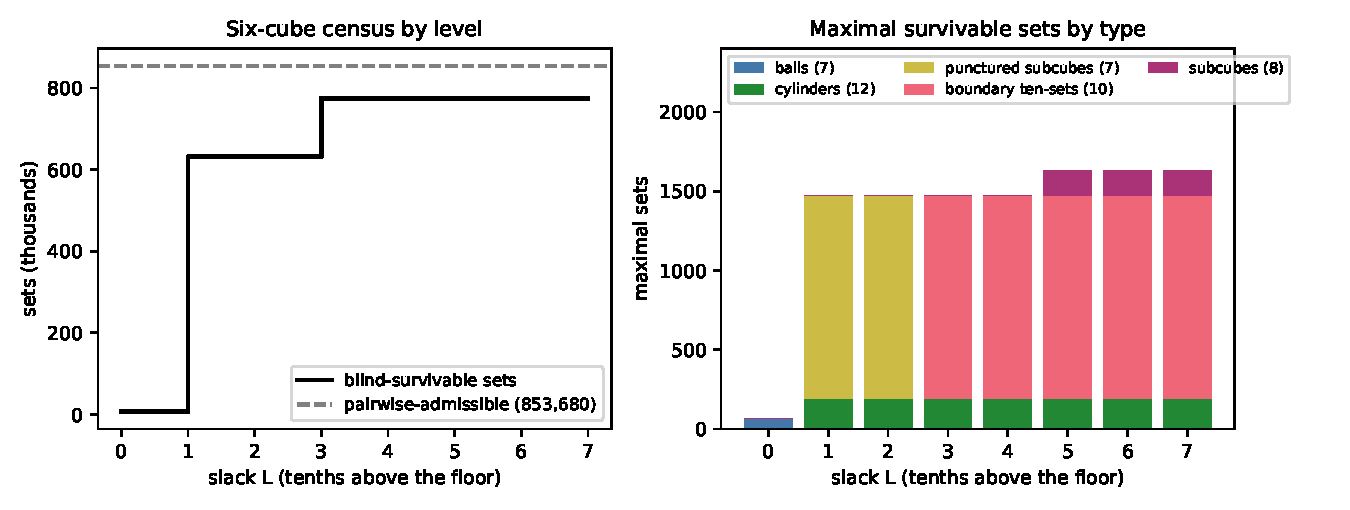
\includegraphics[width=\textwidth]{fig_census.pdf}
\caption{The census of the six-cube by level: survivable sets (left axis, thousands) and maximal sets by type (right axis). The jumps at $L=1$, $3$ and $5$ are the thresholds of the cylinders and punctured subcubes, the boundary ten-sets, and the full three-dimensional subcubes. The dashed line is the pairwise-admissible family.}
\label{fig:census}
\end{figure}

\paragraph{Kleitman's bound is attained but not by balls.}
At $m=4$ and $m=6$ ($\delta_m$ odd) the extremal sets of Kleitman's theorem are doubled balls of a facet; at $m=5$ ($\delta_m$ even) they are balls. In all three cases the extremal sets are survivable, and at $m=4,6$ from slack $1$ rather than at the floor, because the matched action of one centre costs the cells of the other layer one tenth; Corollary~\ref{cor:kleitman} shows that this holds for every $m$.

\paragraph{The largest sets are not the hardest.}
The thresholds are not monotone in size: the twelve-cell cylinders need slack $1$, the ten-cell boundary sets slack $3$, the eight-cell subcubes slack $5$, and the seven-cell punctured subcubes slack $1$ again. The subcube is expensive because its $2^3$ cells disagree on three coordinates, so every sign action is at distance $3$ from one of them ($D=-5$), whereas the cylinder's cells disagree on one coordinate each with a common five-dimensional centre.

\paragraph{Uniform horizon.}
Every minimal obstruction of the three cubes---far pairs at distance $\delta_m+1$, the tetrahedra of the five-cube, the $2{,}400$ four- and five-cell obstructions of the six-cube---has $V=2$, so Corollary~\ref{cor:horizon} gives the same horizon for all of them.

\begin{corollary}[uniform horizon for $m\le6$]\label{cor:uniform}
For $m\in\{4,5,6\}$, every set that is not blind-survivable loses a cell within $L=10(z_0-1)$ steps from common slack $L$, whatever the blind word; the bound is attained by far pairs at $m=4,6$.
\end{corollary}
\begin{proof}
A non-survivable set contains a minimal obstruction $O$ (Theorem~\ref{thm:criterion}, support bound), and $V(O)=2$ for every minimal obstruction by the enumeration, so $5-2V(O)=1$ and the horizon is $\lfloor L/1\rfloor=L$.
\end{proof}

The corollary gives an exact meaning to the ``bands'' of the earlier editions and to the finite-horizon evaluations of Section~\ref{sec:pbvi}: a set that survives $L+1$ steps from slack $L$ is survivable for ever.
\section{Observation: blind values, the feedback game, the deadline}\label{sec:observation}

\subsection{The blind value of a belief and the probe ladder}
Let $b$ be a probability on the cells (a belief) and $L$ a level. The \emph{blind value} of $b$ is the largest $b$-mass that one blind word can keep alive for ever:
\[\mathcal V_L(b)=\max_{(u_t)}\ b\big(\{\theta:\ \theta\text{ survives }(u_t)\text{ from }L\}\big).\]
\begin{proposition}[antichain formula]\label{prop:antichain}
$\mathcal V_L(b)=\max_{A\in\calS_m(L)}b(A)=\max_{A\in\calM_m(L)}b(A)$.
\end{proposition}
\begin{proof}
The set of cells kept by a word is in $\calS_m(L)$, and every $A\in\calS_m(L)$ is kept by some word; heredity lets the maximum run over $\calM_m(L)$.
\end{proof}
This is the finite-cube form of the antichain formula of \cite{Abaee2026prob}, and it turns the classification of Section~\ref{sec:classification} into a value function: at $m=6$ a belief is evaluated by at most $1{,}632$ sums instead of a search over words. Applied to the uniform belief on a $j$-dimensional subcube---the information class after $m-j$ exact probes of individual parameters---it gives the \emph{probe ladder} of Table~\ref{tab:ladder}. At $m=4$ the values double at each probe ($\tfr1{16},\tfr18,\tfr14,\tfr12,1$ at the floor and $\tfr18,\tfr14,\tfr12,1,1$ from slack $1$), as in the earlier editions; at $m=5$ and $m=6$ the ladder is no longer geometric, because balls and cylinders meet subcubes in $1+j$, $2(1+j')$ or $2^j$ cells according to the level, and the last probe is worth nothing as soon as the remaining class is itself survivable.

\begin{table}[t]
\centering\small
\caption{Probe ladder: blind value of the uniform belief on a $j$-dimensional subcube ($m-j$ parameters probed exactly), by level.}
\label{tab:ladder}
\begin{tabular}{llccccccc}
\toprule
$m$ & levels & $j{=}6$ & $5$ & $4$ & $3$ & $2$ & $1$ & $0$\\
\midrule
4 & $L=0$ & & & $\tfr1{16}$ & $\tfr18$ & $\tfr14$ & $\tfr12$ & $1$\\
4 & $L\ge1$ & & & $\tfr18$ & $\tfr14$ & $\tfr12$ & $1$ & $1$\\
5 & $L\le2$ & & $\tfr3{16}$ & $\tfr5{16}$ & $\tfr12$ & $\tfr34$ & $1$ & $1$\\
5 & $L\ge3$ & & $\tfr3{16}$ & $\tfr5{16}$ & $\tfr12$ & $1$ & $1$ & $1$\\
6 & $L=0$ & $\tfr7{64}$ & $\tfr3{16}$ & $\tfr5{16}$ & $\tfr12$ & $\tfr34$ & $1$ & $1$\\
6 & $1\le L\le4$ & $\tfr3{16}$ & $\tfr5{16}$ & $\tfr12$ & $\tfr78$ & $1$ & $1$ & $1$\\
6 & $L\ge5$ & $\tfr3{16}$ & $\tfr5{16}$ & $\tfr12$ & $1$ & $1$ & $1$ & $1$\\
\bottomrule
\end{tabular}
\end{table}

\subsection{The feedback game}
When the stock is observed, an action $u$ played in the information class $T$ reveals $D(u,\theta)$, hence $\dH(u,\theta)$, and splits $T$ into the classes $T_k=\{\theta\in T:D(u,\theta)=k\}$; each class then continues from its own slack $L+k$ with its own words. Survival of the \emph{true} cell, whichever it is, requires every class to be kept.
\begin{definition}[feedback survivability]
$F(T,L)$ holds iff $L\ge\Lstar(T)$, or there is an action $u$ that splits $T$ into at least two classes with $L+k\ge0$ and $F(T_k,L+k)$ for every class. The \emph{feedback threshold} $\Fstar(T)$ is the least $L$ with $F(T,L)$.
\end{definition}
Non-splitting actions need not be considered: one with nonnegative drift on all of $T$ places $T$ inside a ball, where $F$ already holds, and one with negative drift only lowers the slack. The recursion is finite (classes shrink) and is evaluated exactly with memoisation and the certified blind thresholds.

\begin{proposition}[feedback thresholds]\label{prop:feedback}
At $m=4$: $\Fstar(\Theta_4)=23$; for the $j$-dimensional subcubes $\Fstar=1,6,14$ ($j=1,2,3$); for the distance shells of a first action, $\Fstar=0,14,18,14,0$ (shells $h=0,\dots,4$). At $m=5$: $\Fstar(\Theta_5)=18$; subcubes $\Fstar=0,3,7,11$ ($j=1,\dots,4$); shells $\Fstar=0,0,11,11,0,0$. In both cubes $\Lstar(\Theta_m)=\infty$.
\end{proposition}
The whole four-cube is thus kept from $z_0=3.3$ with the stock observed, against never without observation; the price decomposes along the first split, which must be a sign action (the hold reveals nothing): the antipode of the first guess loses $2m+5$ tenths ($13$ at $m=4$) and the far shells, which are not blind-survivable, need $14$ and $18$ more after losing $9$ and $5$, whence $\max(13,\,9+14,\,5+18,\,1+14)=23$. At $m=5$ the shells at distance $1$ and $4$ are spheres of radius one, inside balls, and cost nothing further, so the two ten-cell shells decide: $\Fstar=\max(15,\ 3+11,\ 7+11,\ 11)=18$. The feedback thresholds are the exact ``price of observation'' on the cube; they are new to this edition and are checked by the script.

\begin{figure}[t]
\centering
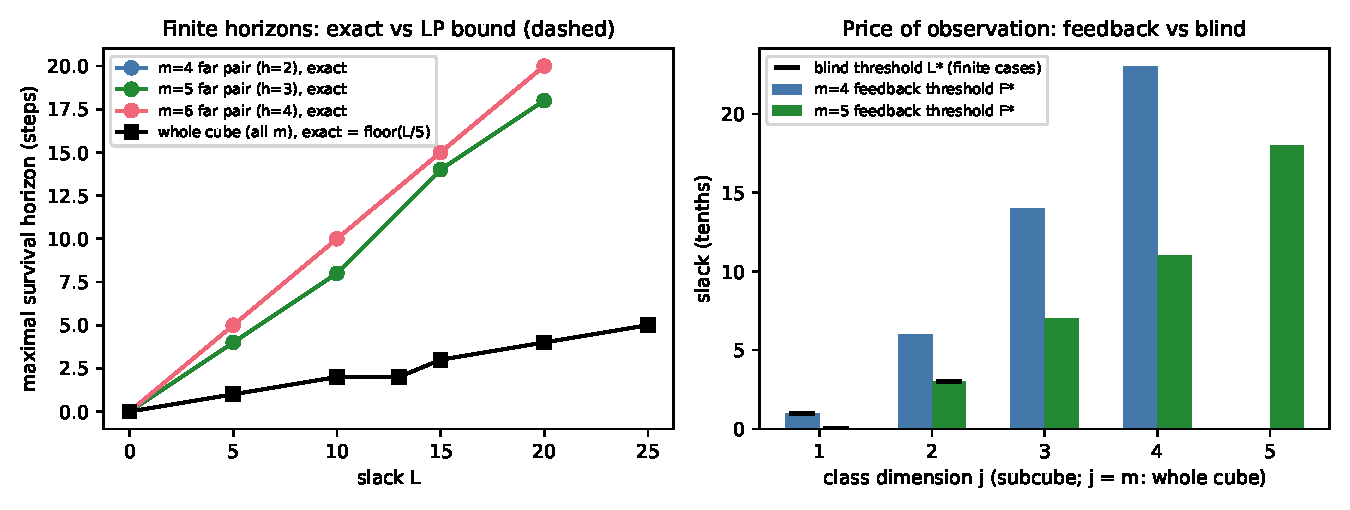
\includegraphics[width=\textwidth]{fig_horizon.pdf}
\caption{Left: maximal survival horizon of the far pairs at distance $\delta_m+1$ ($m=4,5,6$; the $m=4$ and $m=6$ lines coincide with the bound $L$) and of the whole cube (squares, $\lfloor L/5\rfloor$ for every $m$) against the slack $L$; dashed lines are the bound $\lfloor L/(5-2V)\rfloor$ of Corollary~\ref{cor:horizon}. Right: the price of observation---feedback threshold $\Fstar$ of the $j$-dimensional subcubes and of the whole cube ($j=m$) at $m=4,5$, with the blind threshold $\Lstar$ marked where it is finite.}
\label{fig:horizon}
\end{figure}

\subsection{Total ignorance and the deadline}
\begin{proposition}[deadline law]\label{prop:deadline}
From common slack $L$ the whole cube can be kept for exactly $\lfloor L/5\rfloor$ steps and no more, by any blind word; the hold attains this. Equivalently, surviving $T$ periods without any information requires $z_0\ge1+T/2$, for every schedule.
\end{proposition}
\begin{proof}
$V(\Theta_m)=0$ with the uniform certificate ($\sum_\theta\theta=0$), so Corollary~\ref{cor:horizon} gives at most $\lfloor L/5\rfloor$ steps; the hold costs exactly $5$ per step; the cell-sum identity gives the same average.
\end{proof}
The earlier editions proved the necessity half only for the hold schedule; the corollary removes that restriction. The forward search confirms the exact horizon $\lfloor L/5\rfloor$ for $L\le25$ at $m=4,5,6$ (Table~S5.3), and the first-split cost $2m+5$ is the second ingredient of $\Fstar$: at $m=4$ no information can be bought before slack $13$, so a deadline of $T\ge3$ periods ($L=15$) and a first split cannot both be afforded below $z_0=2.3$, and the Lean theorem \texttt{deadline\_law} is the four-cube case.
\section{Point-based evaluation and finite horizons}\label{sec:pbvi}

The earlier editions evaluated beliefs ``point-based'': for a horizon $k$, every word $w\in U_m^k$ produces the \emph{outcome mask} $A_k(w,L)=\{\theta:\theta\text{ survives }w\text{ for }k\text{ steps from }L\}$, and the $k$-step value of a belief is $\mathcal V^{(k)}_L(b)=\max_w b(A_k(w,L))$, a maximum of $b$-masses over the \emph{alpha-set} $\calA_k(L)=\{A_k(w,L)\}$ of distinct masks. This is exact for what it computes---$k$-step survival---and the set $\calA_k(L)$ is small: Table~\ref{tab:alpha} gives its size for $k\le4$ at $m=4$ ($17^4=83{,}521$ words, at most $857$ masks) and $m=5$ ($33^4\approx1.19\cdot10^6$ words, at most $15{,}929$ masks), reproducing the counts of the earlier scripts, and for $k\le3$ at $m=6$. What the earlier editions did not make explicit is the relation between $\mathcal V^{(k)}_L$ and the indefinite value $\mathcal V_L$ of Proposition~\ref{prop:antichain}.

\begin{proposition}[finite versus indefinite horizon]\label{prop:pbvi}
$\mathcal V^{(k)}_L(b)\ge\mathcal V^{(k+1)}_L(b)\ge\mathcal V_L(b)$ for all $k$, with $\mathcal V^{(k)}_L=\mathcal V_L$ for every belief as soon as every mask of $\calA_k(L)$ is in $\calS_m(L)$. For $m\le6$ this holds for $k\ge L+1$ (Corollary~\ref{cor:uniform}). At $m=4,6$ it fails for every $k\le L$ when $L\ge1$, because a far pair at distance $\delta_m+1$ survives exactly $L$ steps; at $m=5$ the longest survival of a non-survivable set is $2\lfloor(L-1)/2\rfloor$ steps (far pairs at distance $3$ and tetrahedra alike, Section~\ref{sec:criterion}), so the point-based value is exact precisely for $k>2\lfloor(L-1)/2\rfloor$: with $k=4$ this is $L\le4$ at $m=5$ against $L\le3$ at $m=4$.
\end{proposition}

Table~\ref{tab:alpha} also reports, for each horizon, how many masks are survivable sets: at $m=4$ and $L=15$ none of the $89$ two-step or $321$ three-step masks is, and $48$ of the $545$ four-step masks are, so a four-step evaluation at $z_0=2.5$ still contains $497$ masks that describe transient survival only. The supplement (S6) tabulates $\mathcal V^{(k)}_L$ for $k=1,\dots,4$ and $\mathcal V_L$ at probed beliefs---the uniform belief, five random beliefs drawn with a fixed seed, and three adversarial beliefs concentrated on a far pair, on an antipodal pair, and on a ball together with its antipode---at every level $L=0,\dots,15$. Three readings: for the uniform belief at $m=4$ the four-step value is $\tfr12$ at $L=15$ ($8$ of $16$ cells survive four steps) while the indefinite value is $\tfr18$ at every $L\ge1$; for the far-pair belief the four-step value is $1$ for every $L\ge4$ and the indefinite value $\tfr12$ at every level; at $m=5$ the uniform four-step value at $L=15$ is $\tfr12$ against $\tfr3{16}$. For $L\le3$ at $m=4$ and $L\le4$ at $m=5$ the finite and indefinite values agree for every probed belief, as Proposition~\ref{prop:pbvi} predicts, and they part at the next level. The point is structural: finite-horizon alpha-sets are exact evaluations of a different quantity, and the horizon at which they become exact for indefinite survival grows with the slack ($L+1$ at $m=4,6$, $2\lfloor(L-1)/2\rfloor+1$ at $m=5$); it is not $4$.

\begin{table}[t]
\centering\small
\caption{Size of the alpha-set $\calA_k(L)$ (distinct $k$-step outcome masks over all words), and in parentheses the number of those masks that are blind-survivable sets, for $k=4$ ($m=4,5$) and $k=3$ ($m=6$); the full $k=1,\dots,4$ tables are S6.1--S6.2.}
\label{tab:alpha}
\begin{tabular}{rlll}
\toprule
$L$ & $m=4$, $k=4$ & $m=5$, $k=4$ & $m=6$, $k=3$\\
\midrule
0 & 17 (16) & 945 (944) & 5{,}281 (5{,}280)\\
1 & 49 (48) & 945 (944) & 11{,}953 (11{,}952)\\
2 & 49 (48) & 945 (944) & --\\
3 & 49 (48) & 1{,}345 (1{,}344) & 33{,}649 (18{,}224)\\
4 & 209 (48) & 1{,}505 (1{,}504) & --\\
5 & 161 (48) & 5{,}265 (1{,}504) & 27{,}409 (13{,}584)\\
6 & 161 (48) & 5{,}265 (1{,}504) & --\\
7 & 185 (48) & 3{,}505 (1{,}344) & --\\
8 & 361 (48) & 6{,}065 (1{,}664) & --\\
9 & 297 (48) & 9{,}625 (1{,}664) & --\\
10 & 249 (48) & 7{,}705 (1{,}664) & 16{,}077 (2{,}144)\\
11 & 249 (48) & 6{,}937 (1{,}536) & --\\
12 & 857 (48) & 14{,}649 (1{,}696) & --\\
13 & 793 (48) & 15{,}929 (1{,}216) & --\\
14 & 729 (48) & 12{,}937 (1{,}104) & --\\
15 & 545 (48) & 11{,}145 (1{,}072) & 24{,}921 (0)\\
\bottomrule
\end{tabular}
\end{table}

\paragraph{What is superseded.} The auxiliary counts of the earlier editions---the number of two-cell supports met in a four-step evaluation, the reduction ``$17^4\to857$''---are properties of $\calA_4(L)$ and remain correct as such; the classification of Section~\ref{sec:classification} replaces them as the statement about survival. All $120$ pairs of the four-cube are now classified by distance ($32$ adjacent and survivable, $48$ at distance $2$, $32$ at distance $3$, $8$ antipodal), and the census tables count sets, not evaluations.
\section{Exact versus floating-point computation, and runtimes}\label{sec:float}

\subsection{Where exactness is needed}
The title of this article and of its predecessors is a claim: exact arithmetic is not what limits belief-state computation on the cube. The classification of Section~\ref{sec:classification} makes the claim precise in both directions. On one side, the whole pipeline---linear programmes, games, census---runs in exact rational arithmetic in minutes (Table~\ref{tab:runtime}). On the other side, the problem contains a large boundary on which floating-point arithmetic gives wrong answers for reasons that no tolerance repairs.

\paragraph{The boundary.}
$143{,}360$ survivable sets of the six-cube, among them the $1{,}280$ maximal ten-sets, have $V(S)=\tfr52$ exactly. For them the decision ``$V\ge\tfr52$'' is an equality test. A floating-point linear programme returned $V=2.5$ with zero error on the representative ten-set (HiGHS \cite{HuangfuHall2018} through SciPy), and so classified it correctly, but only by luck of the rounding: the certificate of correctness is the exact dual $q$, not the float value, and a solver tolerance applied in the wrong direction would reclassify $143{,}360$ sets. The exact simplex of the module costs about five milliseconds on these instances.

\paragraph{The words.}
Proposition~\ref{prop:pinned} says that along every winning word of a boundary set some support cell has slack at most $L$ at every time, and the extracted word of Section~\ref{sec:thresholds} has two cells returning to slack exactly $0$ every four steps. Simulating this word in stock units from $z_0=1.3$ with the floor test $z\ge1$:
\begin{itemize}[leftmargin=2em,itemsep=1pt]
\item in \texttt{float32}, with either coding of the drift, a cell is declared below the floor at step $3$ ($1.3-0.1-0.1-0.1<1$ in single precision), and the deviation from the exact trajectory reaches $11.5$ units after $10^5$ steps for the growing cells;
\item in \texttt{float64} with the drift coded as $-0.5+0.2\,\langle u,\theta\rangle$, no false collapse occurs in $10^5$ steps (maximal deviation $2.7\cdot10^{-8}$);
\item in \texttt{float64} with the drift coded as $(2\langle u,\theta\rangle-5)/10$, the same rational numbers, $1{,}120$ of the $1{,}280$ maximal boundary sets suffer a false collapse within $2{,}000$ steps of their own certified winning words, the earliest at step $3$; the first coding gives none in the same sweep.
\end{itemize}
The verdict of a floating-point simulation on a boundary set therefore depends on the spelling of the drift formula, which is the strongest form of the point made by the title: the \emph{answer} is at a knife edge, so only the arithmetic that represents the edge exactly is admissible. At $m=4$ the adjacent pair from $z_0=1.1$ shows the same touch-the-floor pattern ($1.1\to1.0\to1.3\to1.2\to\dots$) and happens to survive in both \texttt{float64} codings and in \texttt{float32} for $10^5$ steps; luck of this kind is exactly what cannot be relied on.

\begin{figure}[t]
\centering
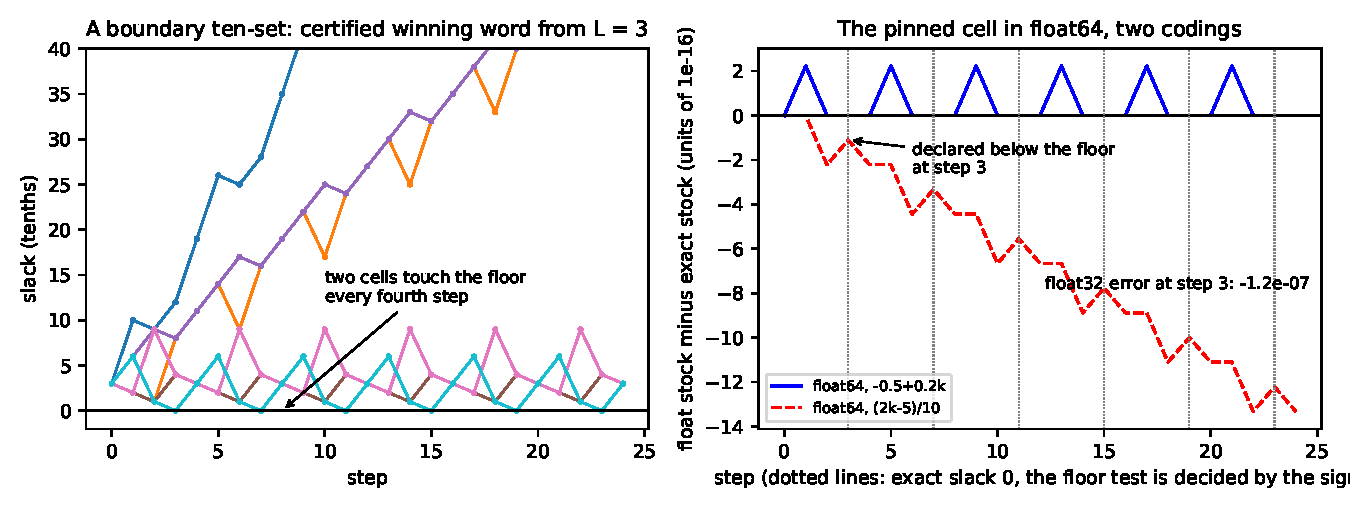
\includegraphics[width=\textwidth]{fig_knife.pdf}
\caption{Left: exact slack trajectories of the ten cells of a boundary ten-set ($V=\tfr52$) under the certified winning word from $\Lstar=3$ (prefix of five actions, period four); two cells return to the floor every fourth step, as Proposition~\ref{prop:pinned} requires. Right: the pinned cell of the second boundary ten-set of the sorted record simulated in \texttt{float64}, shown as the deviation from the exact stock in units of $10^{-16}$ for the two codings of the same drift; dotted lines mark the steps at which the exact slack is $0$, where the floor test is decided by the sign of the rounding error. The coding $(2k-5)/10$ declares the stock below the floor at step $3$; in \texttt{float32} the error at step $3$ is $-1.2\cdot10^{-7}$ under either coding.}
\label{fig:knife}
\end{figure}

\subsection{Runtimes}
\begin{table}[t]
\centering\small
\caption{Wall-clock times of the exact pipeline (single core, Python with exact fractions and NumPy for the bit-mask census). ``Classification'' includes the maximal cliques, the orbit decomposition, all linear programmes, the $5{,}373$ certified subset thresholds of the six-cube and the census; ``point-based'' the alpha-sets for $k\le4$ at $m=4,5$, $k\le3$ at $m=6$, and the obstruction analysis; ``float'' the simulations of Section~\ref{sec:float}.}
\label{tab:runtime}
\begin{tabular}{lr}
\toprule
Stage & seconds\\
\midrule
Classification $m=4,5,6$ (cliques, orbits, LPs, certified thresholds, census) & 147.1\\
Pair tables and horizons & 0.1\\
Observation (ladders, feedback game $m=4,5$, deadline horizons) & 10.1\\
Point-based sweeps and obstructions & 443.9\\
Floating-point study ($10^5$-step simulations, $1{,}280$-set sweep) & 191.7\\
Total & 792.9\\
\bottomrule
\end{tabular}
\end{table}
Table~\ref{tab:runtime} reports the times. The largest items are the six-cube census and the point-based sweeps; the linear programmes themselves are negligible, and the exact game certificates for all $5{,}373$ subsets of the six-cube representatives take under a minute. The earlier editions reported ``four orders of magnitude'' of compression at $m=4$ against the $2^{16}$ power set, which is not the relevant comparison (the admissible family has $48$ members, and the reduction $17^4\to857$ is a count of masks); the relevant statement is that the complete, certified classification of the six-cube, with $2^{64}$ subsets of cells, $853{,}680$ admissible candidates and $774{,}960$ survivable sets, takes two and a half minutes exactly.
\section{Verification record and Lean scope}\label{sec:verification}

\paragraph{Exact module and checks.}
Every number in this article is produced by the exact module \texttt{p05\_core.py} (with the small exact simplex \texttt{exactlp.py}) and the stage scripts \texttt{classify.py}, \texttt{observation.py}, \texttt{pbvi.py}, \texttt{float\_study.py}, assembled by \texttt{run\_all.py} into \texttt{results.json}. The verification script \path{paper05_exact_belief_computation_v20_verification.py} re-derives the theorems' finite content independently of the stored results where that is cheap (drift table, pair values and thresholds, horizons, $m=4$ and $m=5$ classifications, feedback thresholds, deadline horizons, the Lean inventory), checks the stored six-cube record for internal consistency (orbit sizes against the group order, census against threshold histogram, maximal families against the thresholds), and ends with text checks that compare the numbers quoted in the compiled manuscript with \texttt{results.json}; it reports $\NCHECKS$ checks and exits with a nonzero status on any failure. The full run regenerates the six-cube classification ($\approx2.5$ minutes); the \texttt{--quick} mode reuses the stored record. The output of the full run accompanies the manuscript. Tables and figures are generated from \texttt{results.json} by \texttt{make\_si\_tables.py} and \texttt{make\_figs.py}; no table entry is typed by hand.

\paragraph{What the enumeration proves.}
The classifications of Section~\ref{sec:classification} are theorems whose proofs are finite computations with certificates: each linear programme is confirmed exactly on both sides, each threshold on both sides, each orbit by its size. The only non-certified ingredients are the correctness of the Bron--Kerbosch enumeration and of the group action code; both are checked against independent counts (the number of cliques against direct subset enumeration at $m=4,5$, the orbit sizes against the group order).

\paragraph{Lean layer.}
The Lean~4 \cite{MouraUllrich2021} development accompanying the article has eight modules and $80$ theorem declarations with no \texttt{sorry}: \texttt{EBC\_Dynamics} ($28$; the drift, slack and survival definitions in the unscaled model $d=-\tfr12+\tfr15\langle u,\theta\rangle$ over an ordered field with the embedding \texttt{natToK} of the naturals, trajectory algebra), \texttt{EBC\_Hamming} ($6$; agreement mass and Hamming distance, no adjacency triangles in the cube), \texttt{EBC\_Pairs\_v3} ($11$; the pair-sum bound and \texttt{far\_pair\_horizon\_bound}: a far pair survives at most $10(z_0-1)$ steps), \texttt{EBC\_Bands\_v2} ($4$; \texttt{singleton\_survives}), \texttt{EBC\_Classification\_v3} ($5$; \texttt{no\_three\_distinct\_above} and \texttt{survivor\_is\_singleton\_or\_adjacent\_pair}, the four-cube classification from the pair law), \texttt{EBC\_ExactBelief\_v3} ($5$; \texttt{pair\_first\_step\_fails}, the necessity of slack $1$ for adjacent pairs), \texttt{EBC\_Deadline} ($19$; \texttt{deadline\_necessity}, \texttt{deadline\_sufficiency}, \texttt{deadline\_law} for the hold schedule), \texttt{EBC\_Ladder\_v2} ($2$; conditional mass-ratio identities). The repository's Lean audit records the development as compiling with Lean v4.34.1 and Mathlib ($60/60$ jobs); the modules declare no axioms of their own (checked by the verification script), so their theorems depend at most on the standard axioms \texttt{propext}, \texttt{Classical.choice} and \texttt{Quot.sound}. Earlier editions cited sixteen modules and $138$ theorem headers; the present count is of the current, de-duplicated layer.

\paragraph{What is not in Lean.}
The linear criterion (Theorem~\ref{thm:criterion}), the game certificates, the five- and six-cube classifications, the feedback game and the alpha-set statements are proved on paper and by the exact script, not in Lean. The Lean theorems that overlap with this article are the four-cube pair law and classification, the far-pair horizon (the case $m=4$, $h=2$ of Corollary~\ref{cor:horizon}), the first-step necessity for pairs (the case of Proposition~\ref{prop:firststep}) and the hold-schedule half of the deadline law; the article's deadline law for all schedules is Corollary~\ref{cor:horizon} with the uniform certificate and is not formalised. The formal statements are about the unscaled model; the tenths used here are the scaling by $10$, which the module \texttt{EBC\_Bands\_v2} records as \texttt{matched\_drift\_scale\_m4}.
\section{Related work, discussion and open problems}\label{sec:related}

\paragraph{Partially observed control and qualitative POMDPs.}
Keeping a stock above a floor under an unknown but fixed parameter is a safety objective in a partially observable system with a finite, static hidden state. Qualitative analysis of POMDPs---almost-sure and sure safety with belief supports as the relevant state---is the setting of Chatterjee, Doyen and Henzinger \cite{CDH2010}; the blind problem on the cube is the sure-safety problem with a trivial observation function, and the feedback game of Section~\ref{sec:observation} is sure safety with the stock as observation. Point-based value iteration \cite{Pineau2003,Shani2013} and its bounds \cite{Lovejoy1991} approximate quantitative POMDP values on finite horizons; Section~\ref{sec:pbvi} places the exact alpha-sets of the earlier editions in this family and gives the horizon after which finite-horizon survival and indefinite survival coincide ($L+1$ at $m=4,6$; $2\lfloor(L-1)/2\rfloor+1$ at $m=5$). Constrained and chance-constrained POMDPs \cite{Altman1999,Poupart2015,Santana2016,Undurti2010,Ono2015} treat the floor as a constraint in expectation or in probability; here the constraint is sure, and the survivable-set antichain is the exact object.

\paragraph{Antichains.}
Antichain algorithms for universality, model checking and synthesis \cite{DeWulf2006,DeWulf2008,DoyenRaskin2009,Filiot2009,Filiot2011} exploit the fact that the relevant sets of states are up- or down-closed and representable by their minimal or maximal elements. The slack game of Section~\ref{sec:thresholds} is of this kind on $\N^S$, where Dickson's lemma \cite{Dickson1913} guarantees finite antichains but descending chains of up-sets need not stabilise; the saturated game plus forward reachability is the two-sided replacement used here.

\paragraph{Extremal combinatorics of the cube.}
Kleitman's diameter theorem \cite{Kleitman1966} bounds the size of a set of given diameter in the hypercube and identifies the extremal configurations (balls for even diameter, doubled balls of a facet for odd); Corollary~\ref{cor:kleitman} and Theorem~\ref{thm:m6} show that the survivable sets of the cube are governed by it, and that the extremal sets are survivable for $m\le6$. Sperner theory \cite{Sperner1927,Engel1997} supplies the language of antichains in the Boolean lattice; the isoperimetric and Dedekind-type results cited in earlier editions are not used.

\paragraph{Duality.}
Theorem~\ref{thm:criterion} is a minimax theorem on a product of a box and a simplex, the finite-cube instance of the measure certificates of \cite{Abaee2026minimax}, which rest on Sion's theorem and Helly's bound on certificate support; the support bound $m+1$ of Section~\ref{sec:criterion} is the same Helly number. Adjustable robust optimisation \cite{WeiZhang2024} asks when adapting to revealed uncertainty improves a linear programme; the feedback thresholds of Section~\ref{sec:observation} are an exact instance of such a gap ($\Fstar<\infty=\Lstar$) in a safety rather than optimisation setting. Certified and exact computation in reachability analysis \cite{Althoff2020,Geretti2020} shares the motivation of Section~\ref{sec:float}.

\paragraph{What has changed and what is open.}
This edition replaces the enumerative case analyses of the earlier versions by one criterion with certificates, from which the four- and five-cube results follow and the six-cube classification is new; the observation model is computed rather than named; the alpha-set evaluations are placed; and the floating-point question is answered on the sets where it matters. Four questions remain.
\begin{openproblem}[larger cubes]
For $m=7$ the pair bound is $\delta_7=4$, the floor family consists of the $128$ radius-two balls ($29$ cells) and these are the Kleitman-extremal sets, so the largest survivable sets are known; for $m=8$ the largest are the $8\cdot128$ doubled radius-two balls ($58$ cells, $\Lstar=1$). What is not known is the rest of the classification: the maximal survivable sets that are not extremal (at $m=6$ there are two further orbits, with the boundary ten-sets the more numerous) and the level census. The maximal cliques of $G_7$ and $G_8$ have not been enumerated here, and the orbit-and-certificate method needs a symmetry-aware clique enumeration to scale.
\end{openproblem}
\begin{openproblem}[uniform horizon]
Every minimal obstruction found for $m\le6$ has $V=2$. Is $V(O)\le2$ for every minimal obstruction and every $m$, so that the horizon $L$ of Corollary~\ref{cor:uniform} is universal? The possible values of $V$ are rationals of bounded denominator (a vertex of a rational polytope with $\pm1$ data), so the question is whether a value in $(2,\tfr52)$ ever occurs.
\end{openproblem}
\begin{openproblem}[feedback at scale]
$\Fstar(\Theta_m)$ is $23$ and $18$ for $m=4,5$. The recursion is exact but exponential in the class size; a closed form, or the asymptotics in $m$, is open, as is the value of information for partial observations of the stock (a floor indicator only).
\end{openproblem}
\begin{openproblem}[formalisation]
Theorem~\ref{thm:criterion} and the game certificates are elementary and finite; their formalisation would make the five- and six-cube classifications verified computations, by reflection on the certificates stored in \texttt{results.json}.
\end{openproblem}

\section*{Acknowledgements}
The author thanks the anonymous referees of the previous edition, whose reports on the census baseline, the observation model, the point-based proposition, the deadline law and the five-cube certification shaped this reconstruction.
\section*{Declarations}
\paragraph{Funding.} None.
\paragraph{Conflicts of interest.} None.
\paragraph{Data availability.} No external data were used; every instance is a finite set of sign vectors defined in the text.
\paragraph{Code availability.} The exact module \texttt{p05\_core.py}, the stage scripts, \texttt{results.json}, the verification script with its output, the figure and table scripts and the Lean modules are publicly available in the repository \url{https://github.com/MIKEAA2020/general-sustainability}; they reproduce every value, certificate, count, figure and tabulated entry reported here.
\paragraph{AI declaration.} Large language models assisted with drafting, code review and iterative revision. The author reviewed and edited all outputs, re-ran all computations, and takes responsibility for the final work.

\begin{thebibliography}{99}\footnotesize

\bibitem{Abaee2026calc} Abaee, A., 2026. An obstruction calculus for viability under incomplete observation. Figshare preprint, version 2. \url{https://doi.org/10.6084/m9.figshare.33716593.v2}.

\bibitem{Abaee2026cert} Abaee, A., 2026. Computational viability certification under incomplete observation: a continuous-to-finite bridge with exact certificates. Companion manuscript, \url{https://github.com/MIKEAA2020/general-sustainability}.

\bibitem{Abaee2026minimax} Abaee, A., 2026. Minimax dual certificates for the common-action obstruction: sparsity, polyhedral recovery, a benchmark law, and the finite review envelope. Companion manuscript, \url{https://github.com/MIKEAA2020/general-sustainability}.

\bibitem{Abaee2026prob} Abaee, A., 2026. Probabilistic sufficiency under partial observation: belief-state safety values, survivable-set antichains, and the exact price of late information. Companion manuscript, \url{https://github.com/MIKEAA2020/general-sustainability}.

\bibitem{Althoff2020} Althoff, M., Bak, S., Bao, Z., Forets, M., Frehse, G., Freire, D., Kochdumper, N., Li, Y., Mitra, S., Ray, R., Schilling, C., Schupp, S., Wetzlinger, M., 2020. ARCH-COMP20 category report: continuous and hybrid systems with linear continuous dynamics. In: \emph{ARCH20, 7th International Workshop on Applied Verification of Continuous and Hybrid Systems}, EPiC Series in Computing 74, 16--48.

\bibitem{Altman1999} Altman, E., 1999. \emph{Constrained Markov Decision Processes}. Chapman \& Hall/CRC, Boca Raton.

\bibitem{BronKerbosch1973} Bron, C., Kerbosch, J., 1973. Algorithm 457: finding all cliques of an undirected graph. \emph{Communications of the ACM} 16(9), 575--577.

\bibitem{CDH2010} Chatterjee, K., Doyen, L., Henzinger, T.A., 2010. Qualitative analysis of partially-observable Markov decision processes. In: \emph{Mathematical Foundations of Computer Science (MFCS 2010)}, Lecture Notes in Computer Science 6281, Springer, 258--269.

\bibitem{DeWulf2006} De Wulf, M., Doyen, L., Henzinger, T.A., Raskin, J.-F., 2006. Antichains: a new algorithm for checking universality of finite automata. In: \emph{Computer Aided Verification (CAV 2006)}, Lecture Notes in Computer Science 4144, Springer, 17--30.

\bibitem{DeWulf2008} De Wulf, M., Doyen, L., Maquet, N., Raskin, J.-F., 2008. Antichains: alternative algorithms for LTL satisfiability and model-checking. In: \emph{Tools and Algorithms for the Construction and Analysis of Systems (TACAS 2008)}, Lecture Notes in Computer Science 4963, Springer, 63--77.

\bibitem{Dickson1913} Dickson, L.E., 1913. Finiteness of the odd perfect and primitive abundant numbers with $n$ distinct prime factors. \emph{American Journal of Mathematics} 35(4), 413--422.

\bibitem{DoyenRaskin2009} Doyen, L., Raskin, J.-F., 2009. Antichains for the automata-based approach to model-checking. \emph{Logical Methods in Computer Science} 5(1), paper 5.

\bibitem{Engel1997} Engel, K., 1997. \emph{Sperner Theory}. Encyclopedia of Mathematics and its Applications 65, Cambridge University Press, Cambridge.

\bibitem{Filiot2009} Filiot, E., Jin, N., Raskin, J.-F., 2009. An antichain algorithm for LTL realizability. In: \emph{Computer Aided Verification (CAV 2009)}, Lecture Notes in Computer Science 5643, Springer, 263--277.

\bibitem{Filiot2011} Filiot, E., Jin, N., Raskin, J.-F., 2011. Antichains and compositional algorithms for LTL synthesis. \emph{Formal Methods in System Design} 39, 261--296.

\bibitem{Geretti2020} Geretti, L., Alexandre dit Sandretto, J., Althoff, M., Benet, L., Chapoutot, A., Chen, X., Collins, P., Forets, M., Freire, D., Immler, F., Kochdumper, N., Sanders, D.P., Schilling, C., 2020. ARCH-COMP20 category report: continuous and hybrid systems with nonlinear dynamics. In: \emph{ARCH20, 7th International Workshop on Applied Verification of Continuous and Hybrid Systems}, EPiC Series in Computing 74, 49--75.

\bibitem{HuangfuHall2018} Huangfu, Q., Hall, J.A.J., 2018. Parallelizing the dual revised simplex method. \emph{Mathematical Programming Computation} 10(1), 119--142.

\bibitem{Kleitman1966} Kleitman, D.J., 1966. On a combinatorial conjecture of Erd\H{o}s. \emph{Journal of Combinatorial Theory} 1(2), 209--214.

\bibitem{Lovejoy1991} Lovejoy, W.S., 1991. Computationally feasible bounds for partially observed Markov decision processes. \emph{Operations Research} 39(1), 162--175.

\bibitem{MouraUllrich2021} de Moura, L., Ullrich, S., 2021. The Lean 4 theorem prover and programming language. In: \emph{Automated Deduction -- CADE 28}, Lecture Notes in Computer Science 12699, Springer, 625--635.

\bibitem{Ono2015} Ono, M., Pavone, M., Kuwata, Y., Balaram, J., 2015. Chance-constrained dynamic programming with application to risk-aware robotic space exploration. \emph{Autonomous Robots} 39, 555--571.

\bibitem{Pineau2003} Pineau, J., Gordon, G., Thrun, S., 2003. Point-based value iteration: an anytime algorithm for POMDPs. In: \emph{Proceedings of the 18th International Joint Conference on Artificial Intelligence (IJCAI 2003)}, 1025--1032.

\bibitem{Poupart2015} Poupart, P., Malhotra, A., Pei, P., Kim, K.-E., Goh, B., Bowling, M., 2015. Approximate linear programming for constrained partially observable Markov decision processes. In: \emph{Proceedings of the AAAI Conference on Artificial Intelligence} 29(1), 3342--3348.

\bibitem{Santana2016} Santana, P., Thi\'ebaux, S., Williams, B., 2016. RAO*: an algorithm for chance-constrained POMDPs. In: \emph{Proceedings of the AAAI Conference on Artificial Intelligence} 30(1), 3308--3314.

\bibitem{Shani2013} Shani, G., Pineau, J., Kaplow, R., 2013. A survey of point-based POMDP solvers. \emph{Autonomous Agents and Multi-Agent Systems} 27(1), 1--51.

\bibitem{Sperner1927} Sperner, E., 1927. Ein Satz \"uber Untermengen einer endlichen Menge. \emph{Mathematische Zeitschrift} 27, 544--548.

\bibitem{Undurti2010} Undurti, A., How, J.P., 2010. An online algorithm for constrained POMDPs. In: \emph{2010 IEEE International Conference on Robotics and Automation (ICRA)}, 3966--3973.

\bibitem{vonNeumann1928} von Neumann, J., 1928. Zur Theorie der Gesellschaftsspiele. \emph{Mathematische Annalen} 100, 295--320.

\bibitem{WeiZhang2024} Wei, N., Zhang, P., 2024. Adjustability in robust linear optimization. \emph{Mathematical Programming} 208, 581--628.

\end{thebibliography}

\end{document}
